\ifx\wholebook\relax\else
\documentclass{report}
\usepackage{times}
\usepackage{epsfig}
\usepackage{alltt}
\usepackage{xspace}
\usepackage{graphicx}
\usepackage{ifpdf}
\usepackage{ifthen}
\usepackage{amsmath}
\usepackage{a4wide}

\graphicspath{{figures/}} 

\ifpdf
\DeclareGraphicsExtensions{.pdf, .jpg, .tif, .png}
\else
\DeclareGraphicsExtensions{.eps, .jpg}
\fi

\newboolean{toseecomment}
\setboolean{toseecomment}{false}
%%change to false to hidde comment 
\newcommand{\comment}[1]{\ifthenelse{\boolean{toseecomment}}{$\blacktriangleright$ \textit{#1}$\blacktriangleleft$}{}}

\newcommand{\commented}[1]{}

\newboolean{seevwspecific}
\setboolean{seevwspecific}{true}
\newcommand{\vwspecific}[1]{\ifthenelse{\boolean{seevwspecific}}{#1}{}}

\newboolean{seecategoryspecific}
\setboolean{seecategoryspecific}{false}
\newcommand{\categoryspecific}[1]{\ifthenelse{\boolean{seecategoryspecific}}{#1}{}}

\newboolean{seestorespecific}
\setboolean{seestorespecific}{true}
\newcommand{\storespecific}[1]{\ifthenelse{\boolean{seestorespecific}}{#1}{}}

\newboolean{seesqueakspecific}
\setboolean{seesqueakspecific}{false}
\newcommand{\squeakspecific}[1]{\ifthenelse{\boolean{seesqueakspecific}}{#1}{}}


\newcommand{\category}[0]
{\ifthenelse{\boolean{seestorespecific}}
	{package\xspace}
	{category\xspace}}

\newcommand{\ct}[1]{\texttt{#1}\xspace}
\newcommand{\stc}[1]{{\small {\sf #1}}\xspace}
\newcommand{\ST}{{\textsc Smalltalk}\xspace}
\newcommand{\tab}{\makebox[4em]{}}
\newcommand{\ttt}[1]{{\tt #1}}
\newcommand{\chev}{\ttt{>>}}
\newcommand{\vw}{VisualWorks\xspace}
\newcommand{\sq}{Squeak\xspace}
\newcommand{\store}{Store\xspace}
\renewcommand{\chaptername}{Exercise}
\newcommand{\exercise}{\vspace{0.2cm}\noindent \textbf{Exercise:}\xspace}

\newsavebox{\fminibox}
\newlength{\fminilength}

% Fait un truc encadre
\newenvironment{fminipage}[1][\linewidth]
  {\setlength{\fminilength}{#1-2\fboxsep-2\fboxrule}
        \begin{lrbox}{\fminibox}\begin{minipage}{\fminilength}}
  { \end{minipage}\end{lrbox}\noindent\fbox{\usebox{\fminibox}}}

% Pareil mais pas encadre (a utiliser pour ne pas couper une fonction

\newenvironment{nminipage}[1][\linewidth]
  {\setlength{\fminilength}{#1}
        \begin{lrbox}{\fminibox}\begin{minipage}{\fminilength}}
  { \end{minipage}\end{lrbox}\noindent\mbox{\usebox{\fminibox}}}

% Un alltt encadre
\newenvironment{falltt}
  {\vspace*{0.3cm}\begin{fminipage}\begin{alltt}}
  {\end{alltt}\end{fminipage}\vspace*{0.3cm}}

% Un alltt pas encadre
\newenvironment{nalltt}
  {\vspace*{0.3cm}\begin{nminipage}\begin{alltt}}
  {\end{alltt}\end{nminipage}\vspace*{0.3cm}}

% Une fonction encadree
\newenvironment{ffonction}[1]
  {\begin{fonction}[#1]
        \begin{fminipage}
\begin{alltt}
\rule{\linewidth}{0.5pt}}
{\end{alltt}\end{fminipage}\end{fonction}}

\newenvironment{codeonepage}
  {\begin{nminipage}\vspace*{0.2cm}\hrule\vspace*{0.1cm}
\begin{alltt}}
  {\end{alltt} \vspace*{-0.2cm}\hrule \vspace*{0.2cm} \end{nminipage}}

\newenvironment{code}
  {\vspace*{0.1cm}\hrule\vspace*{-0.1cm}\begin{alltt}}
  {\end{alltt}\vspace*{-0.2cm}\hrule \vspace*{0.1cm}}



\begin{document}
\fi

\chapter{A Simple Application: A LAN simulation}
\section*{Basic LAN Application }

The purpose of this exercise is to create a basis on writing
future OO programs. We use the knowledge of the previous
exercise to create classes and methods. We work on an
application that simulates a simple \textbf{LAN} network.  We will
create several classes: \ct{Packet, Node, Workstation}, and
\ct{PrintServer}. We start with the simplest version of a LAN,
then we will add new requirements and modify the proposed
implementation to take them into account.

\subsection*{Creating the Class \ct{Node}}

The class \ct{Node} will be the root of all the entities that
form a \ct{LAN}. This class contains the common basic behavior
for all nodes. As a network is defined as basically a linked list
of nodes, a Node should know its next node. A node should be
uniquely identifiable with a name. We represent the name of a node
using a symbol (because symbols are unique in Smalltalk) and the
next node using a node object. It is the node responsibility to
send and receive packets of information.

\begin{code}
Node inherits from Object 
Collaborators: Node and Packet
Responsibility:
name (aSymbol) - returns the name of the node.
hasNextNode - tells if a node has a next node.
accept: aPacket - receives a packet and treat it. 
Per default sends it to the following node.
send: aPacket - sends a packet to the following node.
\end{code}


\exercise  Create a new \category \ct{LAN}, and create a
subclass of \ct{Object} called \ct{Node}, with two instance
variables: \ct{name} and \ct{nextNode}. 

\exercise  Create accessors and mutators for the two instance
variables. Document the mutators to inform users that the argument
passed to \ct{name:} should be a Symbol, and the arguments
passed to \ct{nextNode} should be a node. Define them in a
\ct{private} protocol. Note that a node is identifiable via
its name. Its name is part of its public interface, so you should
move the method name from the \ct{private} protocol to the
\ct{accessing} protocol. \\

\exercise  Define a method called \ct{hasNextNode} that
returns whether the node has a next node or not. \\

\exercise  Create an instance method \ct{printOn:} that puts
the class name and name variable on the argument
\ct{aStream}. Include my next node's name ONLY if there is a
next node (Hint: look at the method \ct{printOn:} from
previous exercise, and consider that the instance variable
\ct{name} is a symbol and \ct{nextNode} is a node). The expected \ct{printOn:} method behavior is described by the following code:

\begin{code}
(Node new 
   name: \#Node1 ; 
   nextNode: (Node new name: \#PC1)) printString

Node named: Node1 connected to: PC1
\end{code}

\exercise  Create a \textbf{class} method \ct{new} and an
\textbf{instance} method \ct{initialize}. Make sure that a new
instance of \ct{Node} created with the new method uses
\ct{initialize} (see previous exercise). Leave
\ct{initialize} empty now (it is difficult to give meaningful
default values for the \ct{name} and \ct{nextNode} of
\ct{Node}. However, subclasses may want to override this
method to do something). 

\exercise  A node has two basic messages to send and receive
packets. When a packet is sent to a node, the node has to accept
the packet, and send it on. Note that with this simple behavior
the packet can loop infinitely in the LAN. We will propose some
solutions to this issue later. To
implement this behavior, you should add a protocol
\ct{send-receive}, and implement the following two methods -in
this case, we provide some partial code that you should complete
in your implementation:

\begin{code}
accept: thePacket
 "Having received the packet, send it on. This is the default
behavior My subclasses will probably override me to do 
something special"\\
    \dots

send: aPacket
"Precondition: self have a nextNode"

"Display debug information in the Transcript, then
send a packet to my following node"

 Transcript show:
   self name printString,
      ' sends a packet to ',
      self nextNode name printString; cr.
\dots
\end{code}

\begin{figure}[htbp]
\begin{center}
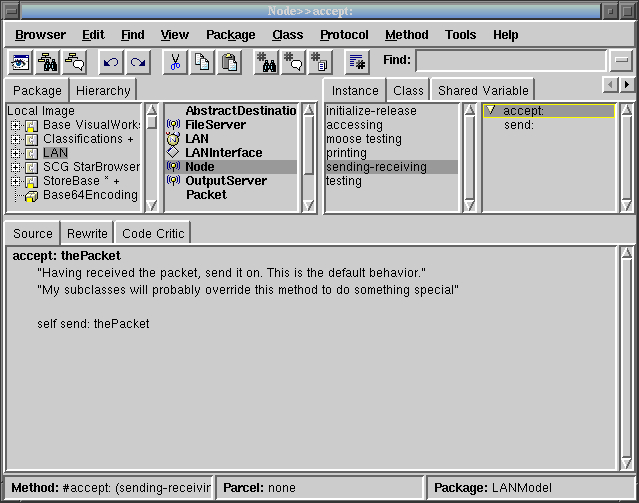
\includegraphics[scale=0.5]{nlesson3Fig1.png}
\caption{nlesson3Fig1.png about here.}
\end{center}
\end{figure}



\subsection*{Creating the Class \ct{Packet}}

A packet in an object that represents a piece of information that is sent from node to node. So the responsibilities of this object are to allow us to define the originator of the sending, the address of the receiver and the contents.

\begin{code}
Packet inherits from Object
Collaborators: Node
Responsibility:
addressee returns the addressee of the node to which 
the packet is sent.
contents - describes the contents of the message sent.
originator - references the node that sent the packet.
\end{code}

\exercise  In the \category LAN, create a subclass of
\ct{Object} called \ct{Packet}, with three instance
variables: \ct{contents}, \ct{addressee}, and \ct{originator}.
Create accessors and mutators for each of them in the
\ct{accessing} protocol (in that particular case the accessors
represents the public interface of the object). The addressee is
represented as a symbol, the contents as a string and the
originator has a reference to a node.

\exercise  Define the method \ct{printOn: aStream} that puts a
textual representation of a packet on its argument
\ct{aStream}.

\subsection*{Creating the Class \ct{Workstation}}

A workstation is the entry point for new packets onto the LAN
network. It can originate packet to other workstations, printers
of file servers. Since it is kind of a network node, but provides
additional behavior, we will make it as a subclass of
\ct{Node}. Thus, it inherits the instance variables and
methods defined in \ct{Node}. Moreover, a workstation have to
manage with packets that are destinated to it in a special way.

\begin{code}
Workstation inherits from Node
Collaborators: Node, Workstation
and Packet
Responsibility: (the ones of node)
originate: aPacket - sends a packet.
accept: aPacket - does some actions on packets sent to the
workstation (printing in the transcript). For the other 
packets just send them to the following nodes.
\end{code}

\exercise In the \category \ct{LAN} create a subclass of
\ct{Node }called \ct{Workstation} without instance
variables. \\

\exercise  Define the method \ct{accept: aPacket} so that if
the workstation is the destination of the packet, the following
message is written into the Transcript. Note that if the packets
are not addressed to the workstation they are sent to the next
node of the current one.

\begin{code}
(Workstation new 
    name: \#Mac ; 
    nextNode: (Printer new name: \#PC1))
          accept: (Packet new addressee: \#Mac)
          
A packet is accepted by the Workstation Mac
\end{code}

\textbf{Hints:} To implement the acceptation of packet addressed
to other node, you could copy and paste the code of the
\ct{Node} class. However this is a bad practice, decreasing
the reuse of code and the ``Say it only once'' rules. It is better
to invoke the default code that is currently overriden by using
\ct{super}. 

\exercise  Write the body for the method \ct{originate:} that
is responsible for inserting packets in the network in the method
protocol \ct{send-receive}. In particular a packet should be
marked with its originator and then sent.

\begin{code}
originate: aPacket
 "This is how packets get inserted into the network.
  This is a likely method to be rewritten to permit 
  packets to be entered in various ways. Currently, 
  I assume that someone else creates the packet and 
  passes it to me as an argument."
 \ldots

\end{code}

\subsection*{Creating the class \ct{LANPrinter}}

\exercise With nodes and workstations, we provide only limited
functionality of a real LAN. Of course, we would like to do
something with the packets that are travelling around the LAN.
Therefore, you will create a class \ct{LanPrinter} here, a
special node that receive packets addressed to it and print them
(on the Transcript). Note that we name it like this because
Printer already exists in the system. Write this class.

\begin{code}
LanPrinter inherits from Node
Collaborators: Node and Packet
Responsibility:
accept: aPacket - if the packet is addressed to the 
printer, prints the packet contents else sends the packet 
to the following node.
print: aPacket - prints the contents of the packet 
(into the Transcript for example).
\end{code}


\subsection*{Simulating the LAN}

Implement the following two methods on the class side of the class
\ct{Node}, in a protocol called \ct{examples}. But take
care the code presented has \textbf{some bugs} that you should
find and fix!.

\begin{code}
simpleLan
  "Create a simple lan"
  "self simpleLan"

 | mac pc node1 node2 igPrinter |

"create the nodes, workstations, printers and fileserver"
mac := Workstation new name: \#mac.
pc := Workstation new name: \#pc.
node1 := Node new name: \#node1.
node2 := Node new name: \#node2.
node3 := Node new name: \#node3.
igPrinter := Printer new name: \#IGPrinter.

"connect the different nodes."
"I make following connections:
\tab \tab mac -\ct{>} node1 -\ct{>} node2 -\ct{>}
\tab \tab igPrinter -\ct{>} node3 -\ct{>} pc -\ct{>} mac"
mac nextNode: node1.
node1 nextNode: node2.
node2 nextNode: igPrinter.
igPrinter nextNode: node3.
node3 nextNode: pc.
pc nextNode: mac.

"create a packet and start simulation"
packet := Packet new
            addressee: \#IGPrinter;
            contents: 'This packet travelled around 
to the printer IGPrinter.

mac originate: packet.
\end{code}

\begin{code}
\textbf{anotherSimpleLan}

"create the nodes, workstations and printers"

{\textbar}mac pc node1 node2 igPrinter node3 packet {\textbar}
mac:= Workstation new name: \#mac.

pc := Workstation new name:\#pc.

node1 := Node new name: \#node1.

node2 := Node new name: \#node2.

node3 := Node new name: \#node3.

igPrinter := LanPrinter new name: \#IGPrinter.

"connect the different nodes." "I make the following connections:
\tab \tab mac -\ct{>} node1 -\ct{>} node2 -\ct{>} \tab
\tab igPrinter -\ct{>} node3 -\ct{>} pc -\ct{>} mac"
mac nextNode: node1.

node1 nextNode: node2.

node2 nextNode:igPrinter.

igPrinter nextNode: node3.

node3 nextNode: pc.

pc nextNode: mac.

"create a packet and start simulation''
packet := Packet new
             addressee: \#anotherPrinter;
             contents: 'This packet travels around 
             to the printer IGPrinter'.
pc originate: packet.
\end{code}


As you will notice the system does not handle loops, we will
propose a solution to this problem in the future. To break the
loop, use or \textbf{Ctrl-Y} depending of the VisualWorks versions.

\subsection*{Creating of the Class \ct{FileServer}}

Create the class \ct{FileServer}, which is a special node that
saves packets that are addressed to it (You should just display a
message on the Transcript).


\begin{code}
FileServer inherits from Node
Collaborators: Node and Packet
Responsibility:
accept: aPacket - if the packet is addressed to the
file server save it (Transcript trace) else send the 
packet to the following node.
save: aPacket - save a packet.
\end{code}

\ifx\wholebook\relax\else\end{document}\fi
